\documentclass[10pt,twocolumn,letterpaper]{article}
\usepackage{cvpr}
\usepackage{times}
\usepackage{graphicx}
\usepackage{amsmath}
\usepackage{amssymb}
\usepackage[pagebackref=true,breaklinks=true,colorlinks,bookmarks=false]{hyperref}
\begin{document}
\title{311-Service-Request Data Analysis using Apache Spark - SOEN 691 Project}
\author{Apoorv Semwal \and Hareesh Kavumkulath \and Loveshant Grewal}
\maketitle

\begin{abstract}
Recent advances in the field of Big Data Analytics and Machine Learning have introduced a plethora of open-source tools and technologies for both, 
academia and the growing data analyst community. In this project we try leveraging one such popular distributed data processing framework Apache Spark
to analyse 311 - Service Request Data for the city of New-York. Being updated almost on a daily basis for the last 10 years, massive size of this dataset makes it a suitable candidate for analysis using a distributed data processing framework like Spark. Making use of Spark Ecosystem libraries like Spark SQL and Spark ML, on this dataset, enables us to derive some interesting insights, which might drive better resource planning within the city. Identifying the 3 primary goals for this project we first try answering a few statistical questions like “most frequent complaints reported(across entire city/borough wise)”, “Average time to resolve the request (category/department wise)”, “mostly used source for making request(borough wise)” and “most busy days/months in terms of request volumes”.
Arriving at these statistical figures involve making extensive use of Spark SQLs Dataframe API. Secondly we generate a model for predicting the closure time for any new incoming service request, after comparing performance of a set of selected supervised learning algorithms available in Spark ML. As part of our last goal we would be applying K-Means clustering over a selected set of features dividing the dataset into clusters to further analyse them for identifying any underlying service request patterns.
\end{abstract}

\section{Introduction}
\subsection{Context}
Open Data movement has now been gaining traction with more of the developed economies realising importance and benefits of releasing general municipal data out in public domain. Within most large cities across the globe, municipalities have been the primary service providers in terms of basic amenities like water, electricity, transportation, infrastructure and public safety. It’s the very nature of their job that requires municipal corporations to handle service request from citizens on a day-to-day basis. Unlike the emergency hotline 911, 311 is the non-emergency public hotline that citizens use for requesting services in regard to the basic municipal or infrastructural issue they face on a day-to-day basis. Given the current rise in data driven decision making practices, this service request data getting accumulated on a daily basis, can eventually prove out to be an incredibly valuable data source for better urban planning. Identifying the general trends in this data would help the authorities identify underlying patterns in the way citizens make requests and make use of it to address issues more proactively.
\subsection{Objective and Problem presentation}
With an overall motivation to offer a small subset of functionalities, a typical decision support tool would provide urban planners and policy makers; we are presenting two primary elements in our project as follows:
\begin{itemize}
\item We first attempt to analyse the 311 service request data for the city of New York and present some statistical insights which would allow urban policy makers to better plan their resources. For instance: 
\begin{itemize}
\item “City wide and Borough wise distribution of most frequently reported complaints”, would help the authorities identify some recurring issues in specific neighbourhoods. As a next step municipal corporations can try addressing the root cause for these recurring issues and analyse if the request pattern is gets reduced over a period of time.   
\item “Most busy days/months in terms of request volumes”, would help the authorities to regulate and plan their resource ahead of time by identifying those specific days or months in a year where they have been receiving higher volume of calls. 
\item “Mostly used source for making request (borough wise)”, would reflect the figures for ease of accessibility to 311 services.   
\item “Average time to resolve the request (request category / department wise)”, as a reflection of how efficient a particular agency or department is in resolving pending requests.  
\item We would end the analysis part by trying to run a clustering algorithm over a selected set of features and analysing the resulting clusters for any specific patterns in neighbourhood based on complaint types.
\end{itemize}
\item Further in this project we try building a predictive model with an ability to predict the closure time for a particular request. This provides greater transparency to citizens and a way for the policy makers to closely scrutinize the operations of the concerned department thereby allowing easy identification of inefficient or ineffective practices, if at all they exist.
\end{itemize}
\subsection{Related Work}
The potential use of Open data towards developing smart cities and improving the delivery of public services has already attracted a massive community of researchers and data enthusiasts. Taking reference of 311-data alone, there exists Open311 [1], a standard protocol developed for civic issue tracking. Developers of the Open311 community even offer a rich set of APIs which are being used to create their independent applications, enabling citizens to conveniently raise and track their 311 requests. In terms of analysis Sam Goodgame and Romulo Manzano from UC Berkeley present a similar analysis of NYC 311 data [2] on an AWS EC2 instance with Hadoop. In [3] authors have gone a step further by combining 311 data for the city of Miami with Census Tracts data and analysing how 311 service request patterns are associated with personal attributes and living conditions. With the existing studies primarily relying on Python libraries like Numpy, Pandas and Scikit Learn, throughout this paper we would be trying to baseline our results against this existing work using an Apache Spark based implementation.

\section{Section 2}

\textbf{1. Sample 1:} Its some random text:
\begin{itemize}
  \item Sample Item 1 \textbf{{\em Sample Italics}} in the dataset.
  \item Sample Item 1 \textbf{{\em Italics}}, 
\end{itemize}

\textbf{2. Sample 2:}\\
\begin{tabular}{ |p{3cm}|p{5cm}|  }
 \hline
 \multicolumn{2}{|c|}{Sample Table} \\
 \hline
 Sample1 &Sample\_1, Sample\_2, Sample\_3\_1\\
 \hline
 Sample1 &Sample\_1, Sample\_2, Sample\_3\_1\\
 \hline
 Sample1 &Sample\_1, Sample\_2, Sample\_3\_1\\
 \hline
\end{tabular}\\

\begin{figure}
   \begin{center}
  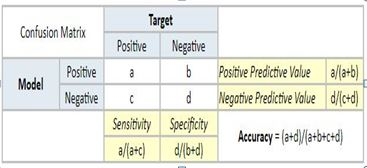
\includegraphics[width=\linewidth]{ConfusionMatrix.JPG}
   \end{center}
   \caption{Sample Confusion Matrix.\cite{W1}
   \label{Img1}}
\end{figure} 
Sample Reference of a figure in text. Figure~\ref{Img1}.\\

\begin{tabular}{ |p{0.5cm}||p{1.4cm}|p{1.4cm}|p{1.4cm}|p{1.4cm}|  }
 \hline
 \multicolumn{5}{|c|}{Multicol Table} \\
 \hline
 ID & Sample2 & Sample3 & Sample4 & Sample5\\
 \hline
 1 & 74.5 & 64.5 & 63.5 & 66.0\\
 \hline
 2 & 78.41 & 81.61 & 81.81 & 82.95\\
 \hline
\end{tabular}\\

\begin{equation}
\frac{\partial Sample Equation_{y_i}}{\partial X}
\end{equation}

\section{Conclusions}
\appendix
{\small
\bibliographystyle{cvpr_bibstyle}
\bibliography{bibliography}
}
\end{document}